The main sources of input information required for a risk calculation with OpenQuake are an exposure model and a physical vulnerability model (in addition to the calculation type, such as those described in Chapter \ref{chap:intrisk}, and the region of interest). An exposure model for a given asset category describes, at each location of interest within a given region, the value of each asset typology. The physical vulnerability model describes the vulnerability characteristics of each asset typology.
%_________________________________________________________
\section{Exposure}
\index{Exposure}
The OpenQuake engine requires an exposure model that needs to be stored according to the respective NRML schema. This file format can include several typologies of asset such as population or buildings. The following parameters are currently being used to describe each asset in the exposure model: 

\begin{itemize}
\item Asset reference: A unique key used to identify the asset instance;
\item Location: Geographic coordinates of the asset expressed in decimal degrees;
\item Asset value: Numerical value of the quantity of the asset at the given location;
\item Vulnerability function: Code of the physical vulnerability function that should be employed in the calculations;
\item Taxonomy: Reference to the classification code that describes the asset.
\end{itemize}

This list of parameters will be further extended in future releases of OpenQuake once more complex data will need to be stored (e.g. value of contents or number of occupants per building at different times of the day).  Furthermore, the definition of the vulnerability function to be used for each asset will be removed from the exposure model, and will instead be stored within a separate file; the two will be linked through the GEM Taxonomy (that is currently under development).

\section{Physical Vulnerability}
\index{Physical Vulnerability}
Physical vulnerability is defined as the probability distribution of loss, given an intensity measure level. These vulnerability functions can be derived directly, usually through empirical methods where the losses from past events at given locations are related to the levels of intensity of ground motion at those locations, or they can be derived by combining fragility functions and consequence functions. Fragility functions describe the probability of exceeding a set of limit states, given an intensity measure level; limit states describe the limits to performance levels, such as damage or injury levels. Fragility functions can be derived by expert-opinion, empirically (using observed data), or analytically, by explicitly modeling the behavior of a given asset typology when subjected to increasing levels of ground motion. Consequence functions describe the probability distribution of loss, given a performance level and are generally derived empirically. 

Version 0.4 of OpenQuake only supports physical vulnerability through the aforementioned vulnerability functions. As part of the Modeller's Toolkit development, calculators that combine fragility functions and consequence functions to produce vulnerability functions will be produced in the future. Furthermore, the possibility to input fragility functions directly is planned in future releases of OpenQuake such that users can view intermediate results of seismic loss calculations, such as the distribution of damage. 

\subsection{Vulnerability Functions}
\subsubsection{Discrete Vulnerability Functions}
\index{Physical Vulnerability!Discrete Functions}
In the current version of OpenQuake (V0.4) discrete vulnerability functions are used to directly estimate fatalities and economic losses due to physical damage. Discrete vulnerability functions are described by a list of intensity measure levels and corresponding mean loss ratios (the ratio of mean loss to exposed value), associated coefficients of variation and probability distributions. The uncertainty on the loss ratio is assumed in OpenQuake v0.4 to follow a lognormal distribution, however different probabilistic distributions for the uncertainty will be developed in future versions, such as the beta distribution. Figure \ref{fig:VFDiscrete} illustrates a discrete vulnerability function.

\begin{figure}[ht]
\centering
\includegraphics[width=10cm,height=6cm]{./Figures/Part_Risk/VFDiscrete.eps}
\caption{Discrete vulnerability function.}
\label{fig:VFDiscrete}
\end{figure}

\subsubsection{Continuous Vulnerability Functions}
\index{Physical Vulnerability!Continuous Functions}
\marginpar{Continuous vulnerability functions are not currently implemented in OQ}
Continuous vulnerability functions will be implemented in future versions of OpenQuake. Continuous vulnerability functions will probably be described by continuous distributions of mean loss ratio and other fractiles of loss ratio, with ground motion intensity. Figure \ref{fig:VFContinuous} illustrates this type of function, showing the distribution of mean loss and the 10 percent and 90 percent fractiles.

\begin{figure}[ht]
\centering
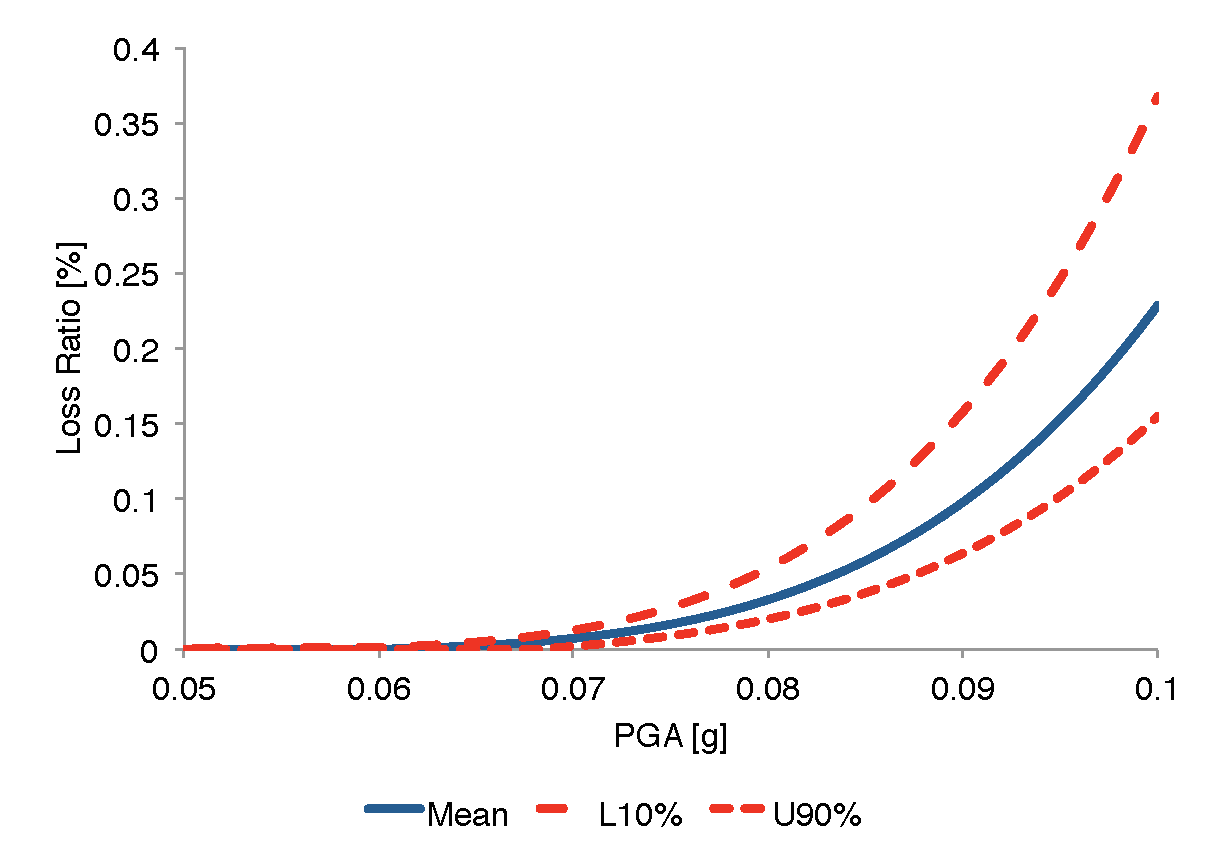
\includegraphics[width=10cm,height=6cm]{./Figures/Part_Risk/VFContinuous}
\caption{Continuous vulnerability function.}
\label{fig:VFContinuous}
\end{figure}

\subsection{Fragility Functions}
\index{Fragility}
\marginpar{Fragility functions are not currently implemented in OQ}
Fragility functions describe the probability of exceeding a set of limit states, given an intensity measure level. When the asset category concerns structures (e.g. buildings), the intensity measure can either be structure-independent or structure-dependent. The former can be calculated directly from recorded measurements of ground shaking (e.g. peak ground acceleration, peak ground velocity, spectral acceleration at a given period of vibration, or even macroseismic intensity). The latter requires information on the characteristics of the structures in order to be calculated, for example spectral acceleration at the fundamental period of vibration, or spectral displacement at the limit state period of vibration. The calculation of these structural characteristics might be through a simple formula (e.g. a yield period-height equation, see e.g. \citet{CrowleyPinho2004} ) or through so-called non-linear static methods, which are needed when the intensity measure is a non-linear response quantity such as spectral displacement at the limit state period of vibration (see e.g. \citet{FEMA440ATC2005}).
Discrete and continuous fragility functions with structure-independent and structure dependent intensity measures (and the methods necessary to calculate them) are not currently supported, but they will be implemented in future versions of OpenQuake. 

\subsubsection{Discrete Fragility Functions}
\index{Fragility!Discrete Functions}
Fragility functions can be defined in a discrete way by providing, for each limit state, a list of intensity measure levels and respective probabilities of exceedance. Figure \ref{fig:FFDiscrete} presents a set of discrete fragility functions using a macroseismic intensity measure. As mentioned previously, these are not yet supported by OpenQuake.

\begin{figure}[ht]
\centering
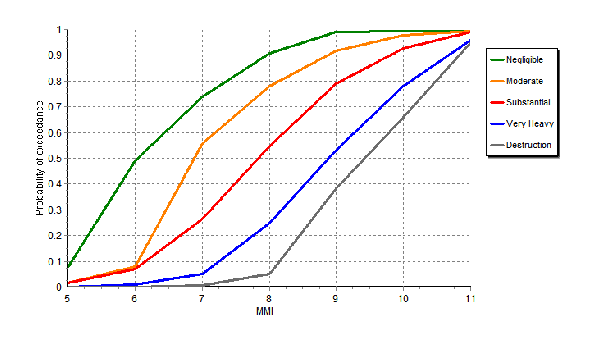
\includegraphics[width=10cm,height=6cm]{./Figures/Part_Risk/FFDiscrete.eps}
\caption{Set of discrete fragility functions.}
\label{fig:FFDiscrete}
\end{figure}

\subsubsection{Continuous Fragility Functions}
\index{Fragility!Continuous Functions}
Continuous fragility functions are defined by the parameters of a cumulative distribution function. In Figure \ref{fig:FFcontinuous} an example of a set of continuous fragility functions with a structure-dependent intensity measure is presented. As mentioned previously, these are not yet supported by OpenQuake.

\begin{figure}[ht]
\centering
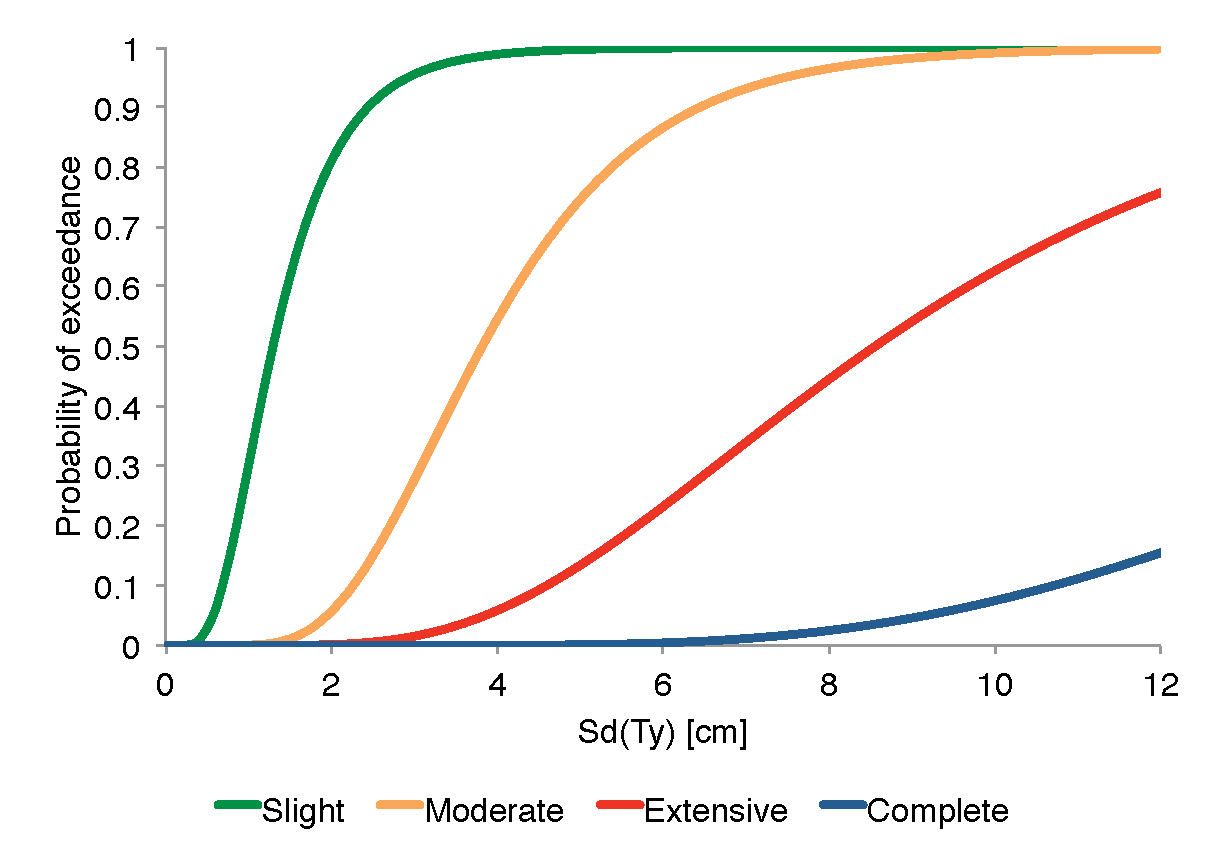
\includegraphics[width=10cm,height=6cm]{./Figures/Part_Risk/FFContinuous.eps}
\caption{Set of continuous fragility functions.}
\label{fig:FFcontinuous}
\end{figure}

\subsubsection{Uncertainty in Fragility Functions}
\index{Fragility!Uncertainty}
The uncertainty in continuous fragility functions will also be accounted for in future versions of OpenQuake. Figure \ref{fig:FF_uncertainty} shows a lognormal distribution that has been fit to the data (i.e. the fragility function), and the probabilistic distribution (i.e. mean and standard deviation) to describe the uncertainty in both the logarithmic mean and logarithmic standard deviation of the fragility function. When a set of fragility functions for different limit states are used, it is also necessary to provide information on the correlation between the logarithmic means and logarithmic standard deviations of each limit state.

\begin{figure}[ht]
\centering
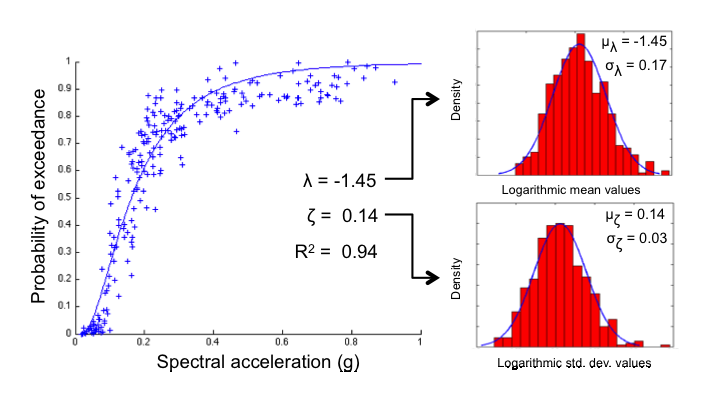
\includegraphics[width=12cm,height=6cm]{./Figures/Part_Risk/FFuncertainty.eps}
\caption{Uncertainty of continuous fragility functions.}
\label{fig:FF_uncertainty}
\end{figure}

\subsection{Consequence Functions}
\index{Consequence Functions}
\marginpar{Consequence functions are not currently implemented in OQ}
Consequence functions describe the probability distribution of loss, given a performance level. For example, if the asset category is buildings and the performance level is significant damage, the consequence function will describe the mean loss ratio, coefficient of variation and probability distribution for that level of damage. Figure \ref{fig:ConsequenceFunctions} presents the mean damage ratios for a set of performance levels proposed by two different sources. 

\begin{figure}[Ht]
\centering
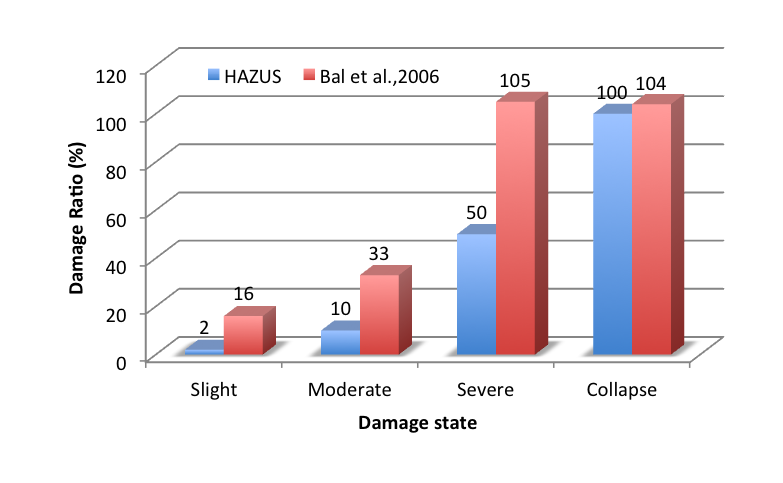
\includegraphics[width=10cm,height=6cm]{./Figures/Part_Risk/ConsequenceFunction.eps}
\caption{Consequence functions adapted from  \citet{Baletal2010}}
\label{fig:ConsequenceFunctions}
\end{figure}

